\documentclass[12pt,a4paper]{extarticle}
\usepackage[left=25mm,right=20mm,top=20mm,bottom=20mm]{geometry}
\usepackage{fontspec}
\IfFontExistsTF{Times New Roman}{\setmainfont{Times New Roman}}{\setmainfont{Liberation Serif}}
\setmonofont{DejaVu Sans Mono}[Scale=0.8]
\usepackage{polyglossia}
\setdefaultlanguage{russian}
\setotherlanguage{english}
\usepackage{amsmath,amssymb,graphicx,booktabs,tabularx,array}
\usepackage{setspace,caption,float,enumitem,titlesec}
\usepackage[unicode,hidelinks]{hyperref}
\hypersetup{pdfauthor={Шешуков Евгений Игоревич},pdflang={ru-RU}}
\setstretch{1.15}
\setlength{\parindent}{1.25cm}
\setlength{\parskip}{3pt}
\setlength{\emergencystretch}{2em}
\setlength{\tabcolsep}{5pt}
\setlength{\intextsep}{8pt}
\renewcommand{\arraystretch}{1.18}
\captionsetup{font=small,labelsep=colon,justification=centering}
\setlist{nosep,topsep=5pt,leftmargin=1.4cm}
\titleformat{\section}{\large\bfseries}{\thesection.}{0.5em}{}
\titleformat{\subsection}{\normalsize\bfseries}{\thesubsection.}{0.5em}{}
\titlespacing*{\section}{0pt}{12pt}{7pt}
\titlespacing*{\subsection}{0pt}{9pt}{4pt}
\setlength{\abovedisplayskip}{7pt}
\setlength{\belowdisplayskip}{7pt}
\widowpenalty=10000
\clubpenalty=10000
\raggedbottom
\newcommand{\code}[1]{\texttt{\small #1}}
\newcommand{\reporttitle}[2]{%
\hypersetup{pdftitle={Лабораторная работа №#1. #2}}
\begin{titlepage}
\begin{center}
{\bfseries БЕЛОРУССКИЙ ГОСУДАРСТВЕННЫЙ УНИВЕРСИТЕТ\par}
\vspace{4mm}
{\bfseries ФАКУЛЬТЕТ ПРИКЛАДНОЙ МАТЕМАТИКИ\par И ИНФОРМАТИКИ\par}
\vspace{4mm}
Кафедра компьютерных технологий и систем
\vspace{34mm}

{\Large\bfseries ОТЧЁТ ПО ЛАБОРАТОРНОЙ\par РАБОТЕ №#1\par}
\vspace{7mm}
{\Large\bfseries «#2»\par}
\vspace{7mm}
Дисциплина: Компьютерная графика\par
\vspace{3mm}
Номер в списке группы: 13
\end{center}
\vspace{24mm}
\hfill\begin{minipage}{0.57\textwidth}
\textbf{Выполнил:}\par
студент 3 курса 2 группы\par
Шешуков Евгений Игоревич\par
\vspace{6mm}
\textbf{Преподаватель:}\par
Каркоцкий Александр Геннадьевич
\end{minipage}
\vfill
\begin{center}Минск, 2026\end{center}
\end{titlepage}
\setcounter{page}{2}}

\begin{document}
\reporttitle{4}{Алгоритмы отсечения отрезков и многоугольников}

\section{Цель и задание}
Изучить алгоритмы отсечения отрезков и многоугольников и показать их работу на координатной плоскости. Для варианта 13 первая часть выполняется методом Сазерленда и Коэна с явным уравнением прямой. Во второй части выпуклый многоугольник отсекается методом Сазерленда и Ходжмана. Отсекающее окно, исходные фигуры и видимые части выделяются разными цветами.

\section{Алгоритмы}
\subsection{Отсечение отрезка прямоугольным окном}
Для каждой точки вычисляется четырёхбитный код. Биты от младшего к старшему соответствуют условиям $x<x_{\min}$, $x>x_{\max}$, $y<y_{\min}$ и $y>y_{\max}$. Точка на границе не получает бит этой границы. Если $c_A\mathbin{\mathrm{OR}}c_B=0$, виден весь текущий отрезок. Если $c_A\mathbin{\mathrm{AND}}c_B\ne0$, оба конца лежат за одной границей и отрезок отбрасывается.

Иначе выбирается внешний конец. Прямая исходного отрезка при $x_0\ne x_1$ задаётся явно уравнением $y=y_0+k(x-x_0)$, где $k=(y_1-y_0)/(x_1-x_0)$. Для вертикальной границы $x=x_b$ вычисляется $y=y_0+k(x_b-x_0)$. Для горизонтальной границы $y=y_b$ вычисляется $x=x_0+(y_b-y_0)/k$. У вертикальной прямой $x=x_0$. Горизонтальный отрезок либо лежит в допустимой полосе по $Y$, либо отбрасывается до вычисления пересечения с горизонтальной границей. После замены конца вычисляются новые коды. Метод выполняет ограниченное число шагов для каждого отрезка, поэтому обработка $n$ отрезков занимает $O(n)$ времени.

\subsection{Отсечение выпуклого многоугольника}
Обрабатываем рёбра выпуклого окна по порядку. Для ориентированного ребра $AB$ знак векторного произведения задаёт полуплоскость, в которой лежит точка $P$:
\[
 d(P)=\sigma\big((B_x-A_x)(P_y-A_y)-(B_y-A_y)(P_x-A_x)\big),
\]
где $\sigma=1$ при обходе окна против часовой стрелки и $\sigma=-1$ при обратном обходе. Внутренними считаются точки с $d(P)\ge0$. Для каждой пары соседних вершин $P,Q$ текущего контура:
\begin{itemize}
\item обе внутри: добавить $Q$;
\item выход из окна: добавить только пересечение $I$;
\item вход в окно: добавить $I$, затем $Q$;
\item обе снаружи: пропустить ребро.
\end{itemize}
Если ребро пересекает границу, то $I=P+t(Q-P)$, где $t=d(P)/(d(P)-d(Q))$. Контур после одного прохода становится входом для следующей границы. Одинаковые соседние вершины объединяются. При касании результатом может быть отрезок или точка. Для $m$ вершин и $k$ рёбер окна время самого отсечения составляет $O(k(m+k))$, так как каждое полуплоскостное отсечение выпуклого контура добавляет не более одной вершины. Входная проверка выпуклости проверяет все вершины относительно каждого ребра.

\clearpage
\section{Сопроводительные вычисления}
\subsection{Отрезок $(-10,-4)\to(10,6)$}
Окно задано условиями $-6\le x\le6$, $-3\le y\le5$. Уравнение прямой $y=1+x/2$. При одновременном выходе за две стороны сначала берётся горизонтальная граница. Для первого конца при $y=-3$ получаем $x=-8$. Эта точка остаётся слева от окна, поэтому далее подставляем $x=-6$ и получаем $y=-2$. Для второго конца сначала получаем $(8,5)$, затем $(6,4)$.

\begin{table}[H]
\centering\small
\caption{Изменение кодов и концов отрезка}
\begin{tabular}{rlll}
\toprule
Шаг & Коды до проверки & Граница или решение & Текущий отрезок после шага \\
\midrule
1 & 0101 / 1010 & Нижняя & $(-8,-3)\to(10,6)$ \\
2 & 0001 / 1010 & Левая & $(-6,-2)\to(10,6)$ \\
3 & 0000 / 1010 & Верхняя & $(-6,-2)\to(8,5)$ \\
4 & 0000 / 0010 & Правая & $(-6,-2)\to(6,4)$ \\
5 & 0000 / 0000 & Принят & $(-6,-2)\to(6,4)$ \\
\bottomrule
\end{tabular}
\end{table}

Из шести отрезков в примере видимы пять. У отрезка $(-9,3)\to(-7,6)$ оба конца имеют бит 0001, поэтому он целиком отбрасывается. Отрезок $(-10,0)\to(-6,4)$ касается левой границы в точке $(-6,4)$.

\subsection{Многоугольник и прямоугольное окно}
Исходный контур проходит через $(-8,-2)$, $(0,-6)$, $(8,-2)$ и $(0,6)$. Окно задано вершинами $(-4,-3)$, $(5,-3)$, $(5,4)$ и $(-4,4)$. Для нижнего ребра окна $d(P)=9(P_y+3)$. На ребре $(-8,-2)\to(0,-6)$ получаем $d(P)=9$, $d(Q)=-27$, $t=1/4$. Пересечение имеет координаты $(-6,-3)$.

\begin{table}[H]
\centering\small
\caption{Число вершин после обработки очередного ребра окна}
\begin{tabular}{rlr}
\toprule
Шаг & Ребро & Число вершин \\
\midrule
1 & Нижнее, $y=-3$ & 5 \\
2 & Правое, $x=5$ & 5 \\
3 & Верхнее, $y=4$ & 6 \\
4 & Левое, $x=-4$ & 6 \\
\bottomrule
\end{tabular}
\end{table}
Итоговый контур проходит через вершины $(-4,2)$, $(-4,-3)$, $(5,-3)$, $(5,1)$, $(2,4)$ и $(-2,4)$. Его площадь равна $56.5$. Она получается из площади окна $9\cdot7$ вычитанием площадей двух прямоугольных треугольников с катетами $2,2$ и $3,3$.

\clearpage
\section{Координатная сетка и интерфейс}
Масштаб $s$ одинаков для обеих осей. Для мировой точки $(x,y)$ экранные координаты равны $X=o_x+sx$, $Y=o_y-sy$. Колесо меняет масштаб около курсора, перетаскивание сдвигает изображение. Кнопка «Вписать» показывает исходные фигуры, окно и начало координат.

\begin{figure}[H]
\centering
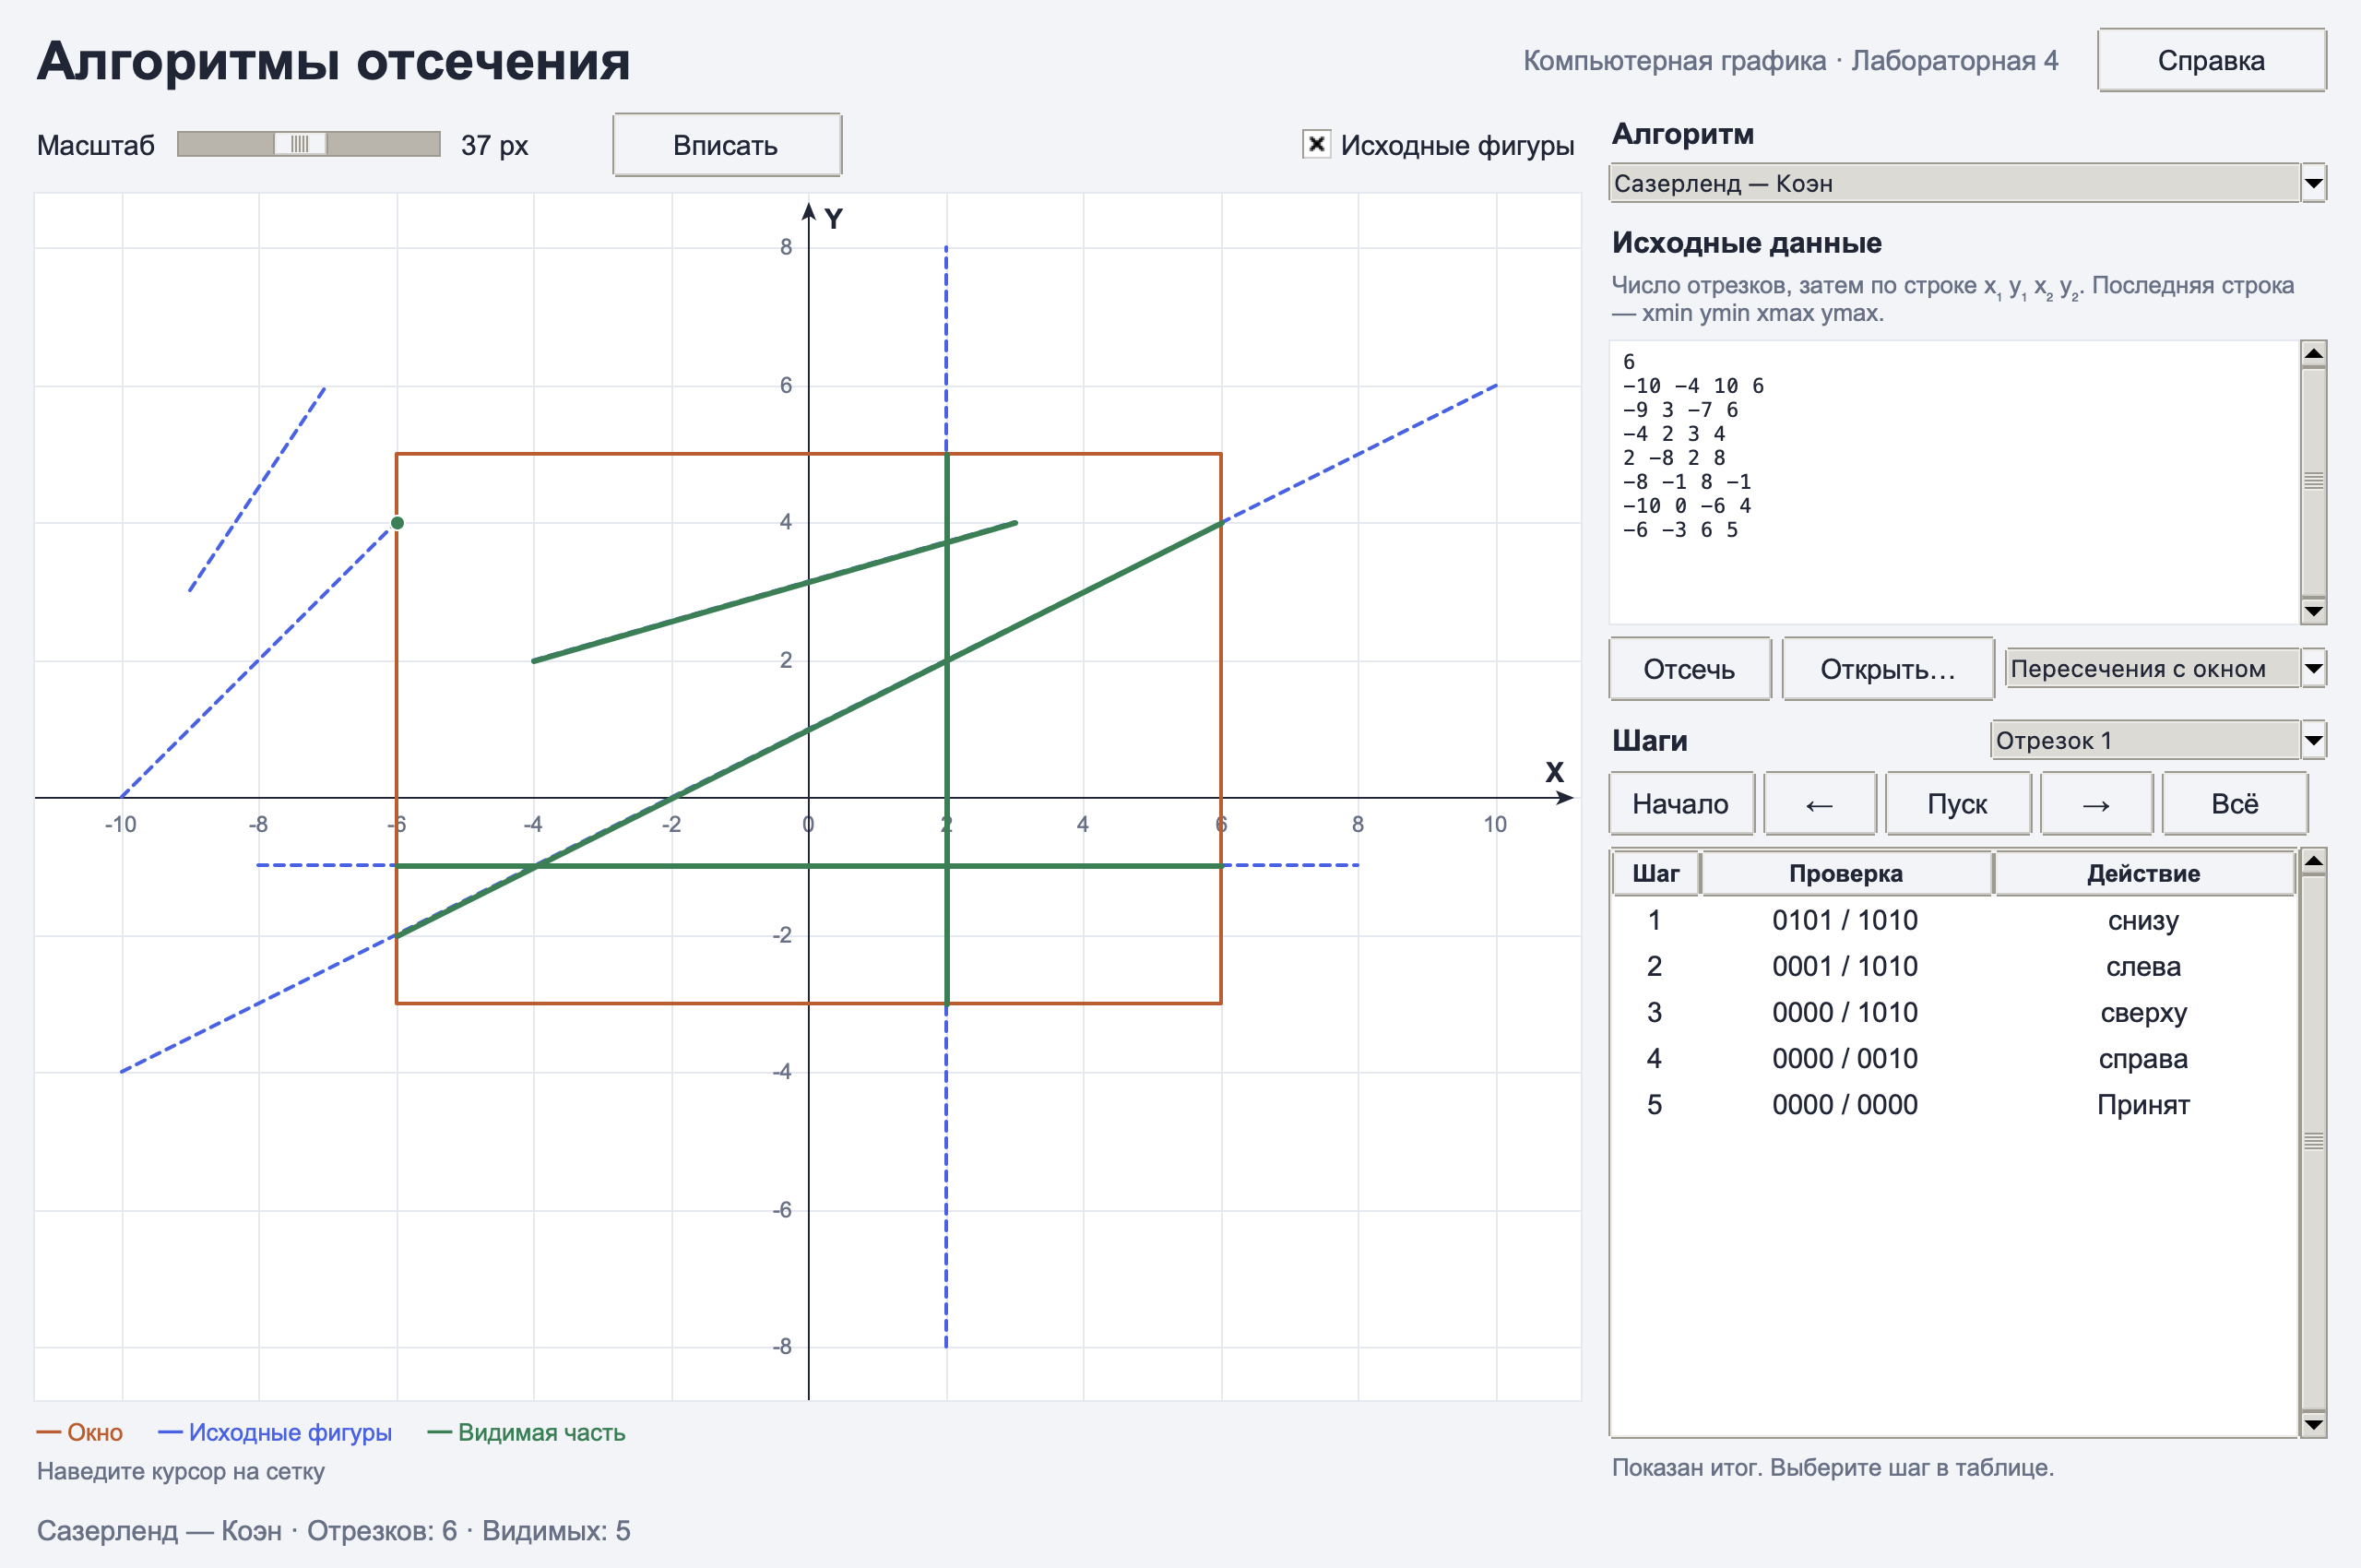
\includegraphics[width=0.80\textwidth]{../docs/segments.png}
\caption{Отсечение отрезков. Справа показаны коды концов первого отрезка}
\end{figure}

\begin{figure}[H]
\centering
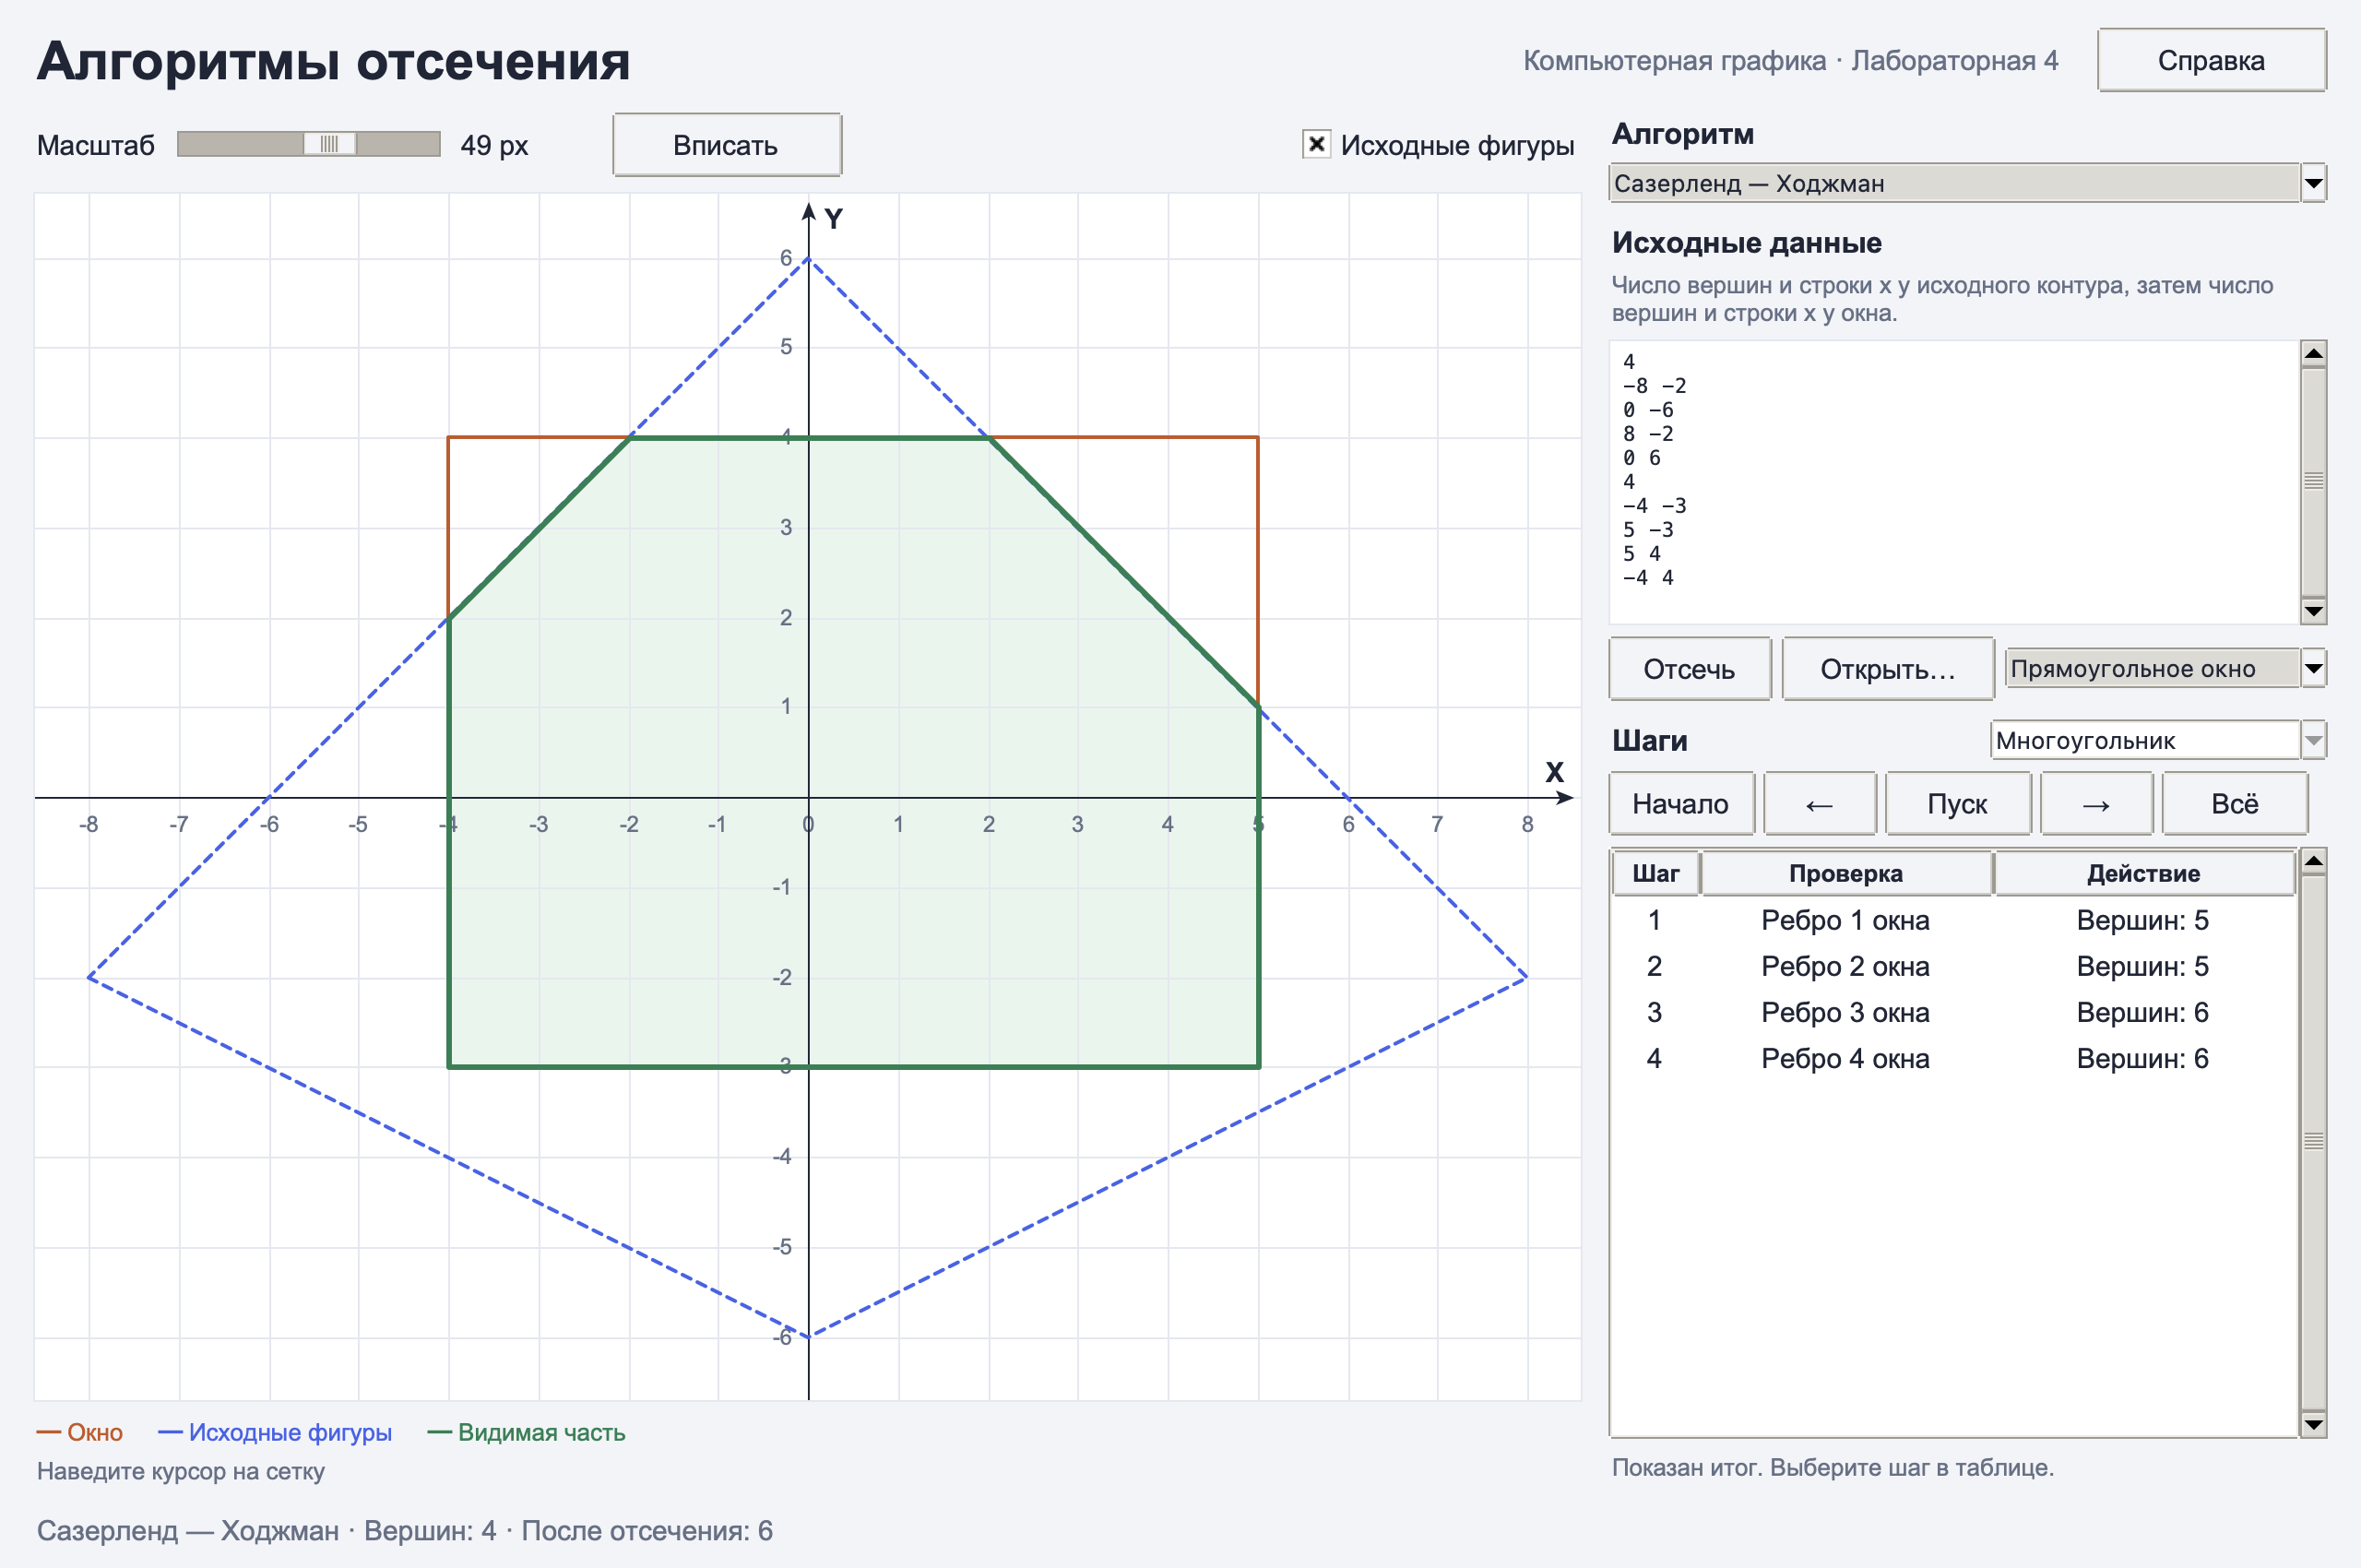
\includegraphics[width=0.80\textwidth]{../docs/polygon.png}
\caption{Исходный контур, прямоугольное окно и видимый многоугольник}
\end{figure}

Оранжевым показано окно, синим пунктиром --- исходные фигуры, зелёным --- видимая часть. Строка таблицы открывает соответствующий шаг. Промежуточная фигура рисуется фиолетовым. Кнопка «Всё» показывает итог.

\clearpage
\section{Реализация, проверка и запуск}
Приложение написано на Python с Tkinter. В файле \code{clipping.py} находятся чтение координат и алгоритмы, в \code{app.py} --- ввод, таблица шагов и отрисовка. Входные десятичные числа и пересечения хранятся как рациональные числа \code{Fraction}. Это позволяет проверять попадание на границу и совпадение вершин точно. При переводе в экранные координаты используются вещественные числа.

Исходные данные можно ввести в редакторе или загрузить из текстового файла. Для отрезков используется формат из условия: число отрезков, по четыре координаты на каждый отрезок и строка с границами прямоугольника. Для многоугольников указываются число вершин и пары $x,y$ исходного контура, затем число вершин и пары $x,y$ окна. Вершины перечисляются по порядку обхода, по часовой стрелке или против неё. Окно во второй части может быть произвольным выпуклым многоугольником. Координаты вводятся от $-1000$ до $1000$ с шестью знаками после десятичной точки или меньшей точностью. При ошибке ввода приложение оставляет предыдущий результат и выводит пояснение.

Пройдено 17 тестов: 11 для вычислений и ввода, 6 для интерфейса. Проверены вертикальные и горизонтальные отрезки, полное отклонение, попадание на границу, касание вершины, наклонное окно и оба направления обхода. Для 500 случайных отрезков результат дополнительно сравнивался с пересечением интервалов параметра. В настоящем окне Tkinter проверены выбор шагов, анимация, чтение файлов, обработка ошибочных данных, масштабирование, сдвиг и отображение при минимальном размере окна.

Для запуска нужно открыть папку \code{labs/lab04} и дважды щёлкнуть по файлу \code{run.command} на macOS или \code{run.bat} на Windows. На macOS файл запуска открывает новые окна приложения без восстановления окон предыдущего сеанса Python. Команда ручного запуска приведена в \code{README.md}. Требуется Python 3.10 или новее с Tkinter. Для пересборки PDF из папки \code{report} выполняется \code{tectonic report.tex}.

\section{Выводы}
Метод Сазерленда и Коэна использует коды концов для полного принятия или отклонения отрезка и находит пересечения с отдельными сторонами прямоугольника. Для разобранного отрезка получена видимая часть $(-6,-2)\to(6,4)$. Метод Сазерленда и Ходжмана последовательно оставляет внутренние полуплоскости окна. В контрольном примере четырёхугольник превращается в шестиугольник площадью $56.5$. Таблица шагов показывает, как меняются коды отрезка и число вершин контура.

\subsection*{Источники}
\begin{enumerate}
\item Условие лабораторной работы №4 «Алгоритмы отсечения отрезков и многоугольников»: \code{assignment.pdf}.
\item J. D. Foley, A. van Dam, S. K. Feiner, J. F. Hughes. \href{https://www.informit.com/store/computer-graphics-principles-practice-9780201121100}{Computer Graphics: Principles and Practice}. 2nd ed., Addison-Wesley, 1990, \S 3.12.
\item I. E. Sutherland, G. W. Hodgman. \href{https://doi.org/10.1145/360767.360802}{Reentrant Polygon Clipping}. Communications of the ACM, 1974, 17(1), 32--42.
\end{enumerate}
\end{document}
